\documentclass[12pt,a4paper]{article}
\usepackage[utf8]{inputenc}
\usepackage[spanish,es-tabla]{babel}
\usepackage{geometry}
\usepackage{graphicx}
\usepackage{multirow}
\usepackage{tabularx}
\usepackage{mathptmx}
\usepackage{fancyhdr}
\usepackage{array}
\usepackage[table]{xcolor}
\usepackage{titlesec}
\usepackage{setspace}
\usepackage{microtype}
\usepackage{lastpage}
\usepackage{booktabs}
\usepackage{enumitem}
\usepackage{amsmath}
\usepackage{amsfonts}
\usepackage{amssymb}

\usepackage{float}
\usepackage{placeins}
\usepackage{tikz}
\usepackage{pgfplots}
\pgfplotsset{compat=1.17}
\usetikzlibrary{arrows.meta,positioning,shapes.geometric,calc}

\graphicspath{{images/}{../images/}{./}}

\geometry{
    top=4.7cm,
    bottom=2.5cm,
    left=2.5cm,
    right=2.5cm,
    headheight=3.9cm,
    headsep=0.4cm
}

\setstretch{1.15}
\setlength{\parindent}{0pt}
\setlength{\parskip}{0.45em}
\setlength{\tabcolsep}{4pt}

\titleformat{\section}
  {\normalfont\fontsize{12}{14.5}\bfseries}{\thesection.}{0.6em}{\uppercase}
\titlespacing*{\section}
  {0pt}{1.8ex plus 0.4ex minus 0.2ex}{0.6ex plus 0.2ex}

\titleformat{\subsection}
  {\normalfont\fontsize{11.5}{13.5}\bfseries}{\thesubsection.}{0.5em}{}
\titlespacing*{\subsection}
  {0pt}{1.4ex plus 0.3ex minus 0.1ex}{0.4ex plus 0.1ex}

\titleformat{\subsubsection}
  {\normalfont\fontsize{10.5}{12.5}\bfseries\itshape}{\thesubsubsection.}{0.4em}{}
\titlespacing*{\subsubsection}
  {0pt}{1.1ex plus 0.2ex minus 0.1ex}{0.3ex plus 0.1ex}

\newcolumntype{Y}{>{\centering\arraybackslash}X}
\newcolumntype{L}{>{\raggedright\arraybackslash}X}
\newcolumntype{C}{>{\centering\arraybackslash}X}

\definecolor{headerblue}{RGB}{26, 54, 93}
\definecolor{darkblue}{RGB}{43, 108, 176}
\definecolor{lightgraybg}{RGB}{248, 248, 248}
\definecolor{tableheader}{RGB}{232, 238, 246}
\definecolor{navyheader}{RGB}{0, 32, 96}
\definecolor{lineblue}{RGB}{0, 102, 204}
\definecolor{areablue}{RGB}{220, 236, 252}
\definecolor{lcsred}{RGB}{217, 56, 41}
\definecolor{lcigreen}{RGB}{46, 125, 50}
\definecolor{lciorange}{RGB}{230, 81, 0}
\definecolor{ishikawared}{RGB}{160, 0, 0}

\tikzset{
    catbox/.style={draw, fill=tableheader, font=\footnotesize\bfseries, minimum width=2.8cm, minimum height=0.65cm, align=center},
    efectobox/.style={draw=ishikawared!90!black, line width=1.2pt, fill=ishikawared, text=white, font=\small\bfseries, align=center, inner sep=6pt, text width=3.8cm},
    causetext/.style={font=\scriptsize, align=right, text=black!90}
}

\newcommand{\docCodigo}{TI-SIGE-ENT-F3-013}
\newcommand{\docVersion}{1.0}
\newcommand{\docProceso}{IMPLEMENTACIÓN DE SOFTWARE / REVISIÓN Y FIRMAS DIGITALES}
\newcommand{\docElaboracion}{06/10/2026}
\newcommand{\docRevision}{06/10/2026}
\newcommand{\docTitulo}{MÓDULO DE REVISIÓN Y CASCADA DE FIRMAS}
\newcommand{\docOrganizacion}{FACULTAD DE INGENIERÍA EN SISTEMAS, ELECTRÓNICA E INDUSTRIAL}
\newcommand{\docSubOrganizacion}{CARRERA DE INGENIERÍA DE SOFTWARE}

\newcommand{\encabezadofrecuente}{%
    \renewcommand{\arraystretch}{1.15}%
    \noindent\makebox[\textwidth][c]{%
    \begin{tabularx}{\textwidth}{|>{\centering\arraybackslash}m{2.8cm}|Y|>{\centering\arraybackslash}m{4.8cm}|}
        \hline
        \multirow{4}{2.8cm}{\centering\raisebox{-1.15cm}{
\includegraphics[width=2.5cm,height=2.0cm,keepaspectratio]{images/logo.png}}}
        & \textbf{\fontsize{9}{11}\selectfont \docOrganizacion} 
        & \textbf{\fontsize{8}{10}\selectfont CÓDIGO:} \fontsize{8}{10}\selectfont \docCodigo \\
        \cline{3-3}
        & \textbf{\fontsize{8.5}{10.5}\selectfont \docSubOrganizacion} 
        & \textbf{\fontsize{8}{10}\selectfont VERSIÓN:} \fontsize{8}{10}\selectfont \docVersion \\
        \cline{2-3}
        & \textbf{\fontsize{8}{10}\selectfont PROCESO:} \fontsize{8}{10}\selectfont \docProceso 
        & \textbf{\fontsize{8}{10}\selectfont ELABORACIÓN:} \fontsize{8}{10}\selectfont \docElaboracion \\
        \cline{2-3}
        & \textbf{\fontsize{8.5}{10.5}\selectfont \docTitulo} 
        & \textbf{\fontsize{8}{10}\selectfont ÚLTIMA REVISIÓN:} \fontsize{8}{10}\selectfont \docRevision \\
        \hline
    \end{tabularx}%
    }%
}

\pagestyle{fancy}
\fancyhf{}
\fancyhead[C]{\encabezadofrecuente}
\fancyfoot[C]{\fontsize{10}{12}\selectfont Página \thepage\ de \pageref{LastPage}}
\renewcommand{\headrulewidth}{0pt}

\begin{document}

\noindent{\fontsize{10.5}{12.5}\selectfont \textbf{Integrantes:} Heidi Villavicencio \quad$\vert$\quad Steeven Toala \quad$\vert$\quad Nixon Hurtado \quad$\vert$\quad Andrea Vásquez}

\vspace{0.25cm}

\section{Título}
\textbf{Denominación Oficial del Entregable:} Módulo de Revisión, Observaciones y Cascada de Firmas -- Código EDT: 3.13

\section{Introducción}
El flujo colegiado de revisión y aprobación de los planes de trabajo del SGC en la FISEI involucra una cadena de responsabilidades jerárquica: el Docente Elaborador diseña el plan, el Coordinador de Área o Carrera audita su coherencia y registra observaciones técnicas, y finalmente las autoridades de facultad (Subdecano / H. Consejo Directivo) legalizan el documento. Para automatizar este flujo con plena validez institucional, se implementó el panel de revisión con panel lateral (\textit{Drawer}) de observaciones granulares por sección y el subsistema de estampado secuencial e inmutable de firmas digitales en cascada (\textit{Cascading Signatures}).

\section{Objetivo}
\subsection{Objetivo General}
Implementar el módulo de revisión técnica colegiada, gestión granular de observaciones y cascada secuencial de firmas digitales para el sistema SIGE.
\subsection{Objetivos Específicos}
\begin{itemize}[leftmargin=1.5em, itemsep=2pt]
    \item Desarrollar el panel de revisión del coordinador con visor de documento y drawer de observaciones.
    \item Programar el sistema de firmas en cascada secuencial inmutable con hash SHA-256 y marca temporal.
    \item Implementar las transiciones de estado: \textit{Borrador} $\to$ \textit{En Revisión} $\to$ \textit{Observado} $\to$ \textit{Aprobado Comisión} $\to$ \textit{Aprobado HCD}.
\end{itemize}

\section{Alcance}
\subsection{Límites del Entregable (In-Scope)}
\begin{itemize}[leftmargin=1.5em, itemsep=2pt]
    \item Interfaz de usuario para Coordinador de Carrera y Comité de Revisión (\texttt{RevisionComiteView.jsx}).
    \item Servicio de firmas digitales en backend garantizando orden estricto (1: Elaborador, 2: Revisor, 3: Aprobador).
    \item Trazabilidad y no repudio de firmas mediante hash de contenido.
\end{itemize}
\subsection{Exclusiones (Out-of-Scope)}
\begin{itemize}[leftmargin=1.5em, itemsep=2pt]
    \item Integración con certificados de firma electrónica con token USB físico (Banco Central / Security Data), prevista para fases de interoperabilidad externa.
\end{itemize}

\section{Definiciones}
\begin{itemize}[leftmargin=1.5em, itemsep=2pt]
    \item \textbf{Cascada de Firmas:} Mecanismo criptográfico y de negocio donde una firma requiere obligatoriamente la existencia y validez de la firma del nivel jerárquico anterior.
    \item \textbf{Observación Granular:} Comentario correctivo vinculado de forma unívoca a una sección específica del documento, que impide su aprobación hasta ser resuelta.
    \item \textbf{Estampillado Digital (Timestamping):} Registro criptográfico inmutable de la fecha, hora exacta e identidad del firmante al momento del visado.
\end{itemize}

\section{Responsabilidades}
\begin{itemize}[leftmargin=1.5em, itemsep=2pt]
    \item \textbf{Steeven Toala (Responsable EDT 3.13):} Desarrollo del servicio de firmas digitales, hashes y control de estados.
    \item \textbf{Heidi Villavicencio (UI/UX):} Diseño e implementación del drawer lateral de observaciones y visor de revisión.
    \item \textbf{Ing. Paulo Torres (Docente Evaluador):} Aprobación del flujo de revisión y cadena de responsabilidades.
\end{itemize}

\section{Normativa Legal y Técnica}
\subsection{Marco Legal Ecuatoriano}
\begin{itemize}[leftmargin=1.5em, itemsep=2pt]
    \item \textbf{Ley de Comercio Electrónico, Firmas Electrónicas y Mensajes de Datos, Art. 14 y 15:} Validez jurídica, eficacia y no repudio de firmas digitales.
    \item \textbf{Ley Orgánica de Educación Superior (LOES), Art. 122:} Responsabilidad institucional de autoridades y docentes en la legalización académica.
\end{itemize}
\subsection{Normas Técnicas Internacionales}
\begin{itemize}[leftmargin=1.5em, itemsep=2pt]
    \item \textbf{ISO 9001:2015, Cláusula 7.5.3 (Control de la información documentada):} Procedimientos de revisión, aprobación y custodia.
    \item \textbf{NIST SP 800-89 (Recommendation for Obtaining Assurances for Digital Signatures).}
\end{itemize}

\section{Método, Políticas y Contenidos}
\subsection{Enfoque Metodológico}
Se diseñó un mecanismo de tres niveles de firma. Cada firma calcula un hash criptográfico compuesto a partir del identificador del documento, el contenido HTML de sus secciones, la identidad del firmante y la estampa de tiempo UTC:
\begin{equation}
    H_{\text{firma}} = \text{SHA-256}\Big(\text{plan\_id} \ \Vert \ H_{\text{contenido}} \ \Vert \ \text{usuario\_id} \ \Vert \ \text{timestamp}\Big)
\end{equation}
Cualquier intento de alteración posterior del texto invalida el hash registrado. El coordinador interactúa a través de una vista dividida (\textit{Split View}): a la izquierda el plan de trabajo A4 y a la derecha el drawer interactivo donde puede marcar secciones como conformes o ingresar observaciones con severidad (Leve, Grave, Bloqueante).

\subsection{Políticas de Calidad de la Cascada de Firmas}
\begin{enumerate}[leftmargin=1.5em, itemsep=2pt]
    \item \textbf{Política de Secuencia Ineludible:} El Coordinador no puede firmar si el Docente no ha firmado; el Subdecano no puede legalizar si el Coordinador no ha aprobado.
    \item \textbf{Política de Congelamiento por Firma:} Al estampar la primera firma, el documento pasa a modo de solo lectura estricto, impidiendo cualquier edición salvo que sea devuelto formalmente a estado ``Observado''.
    \item \textbf{Política de Resolución Obligatoria de Observaciones:} El sistema bloquea el botón de aprobación si existe al menos una observación sin marcar como ``Resuelta''.
\end{enumerate}

\begin{figure}[H]
    \centering
    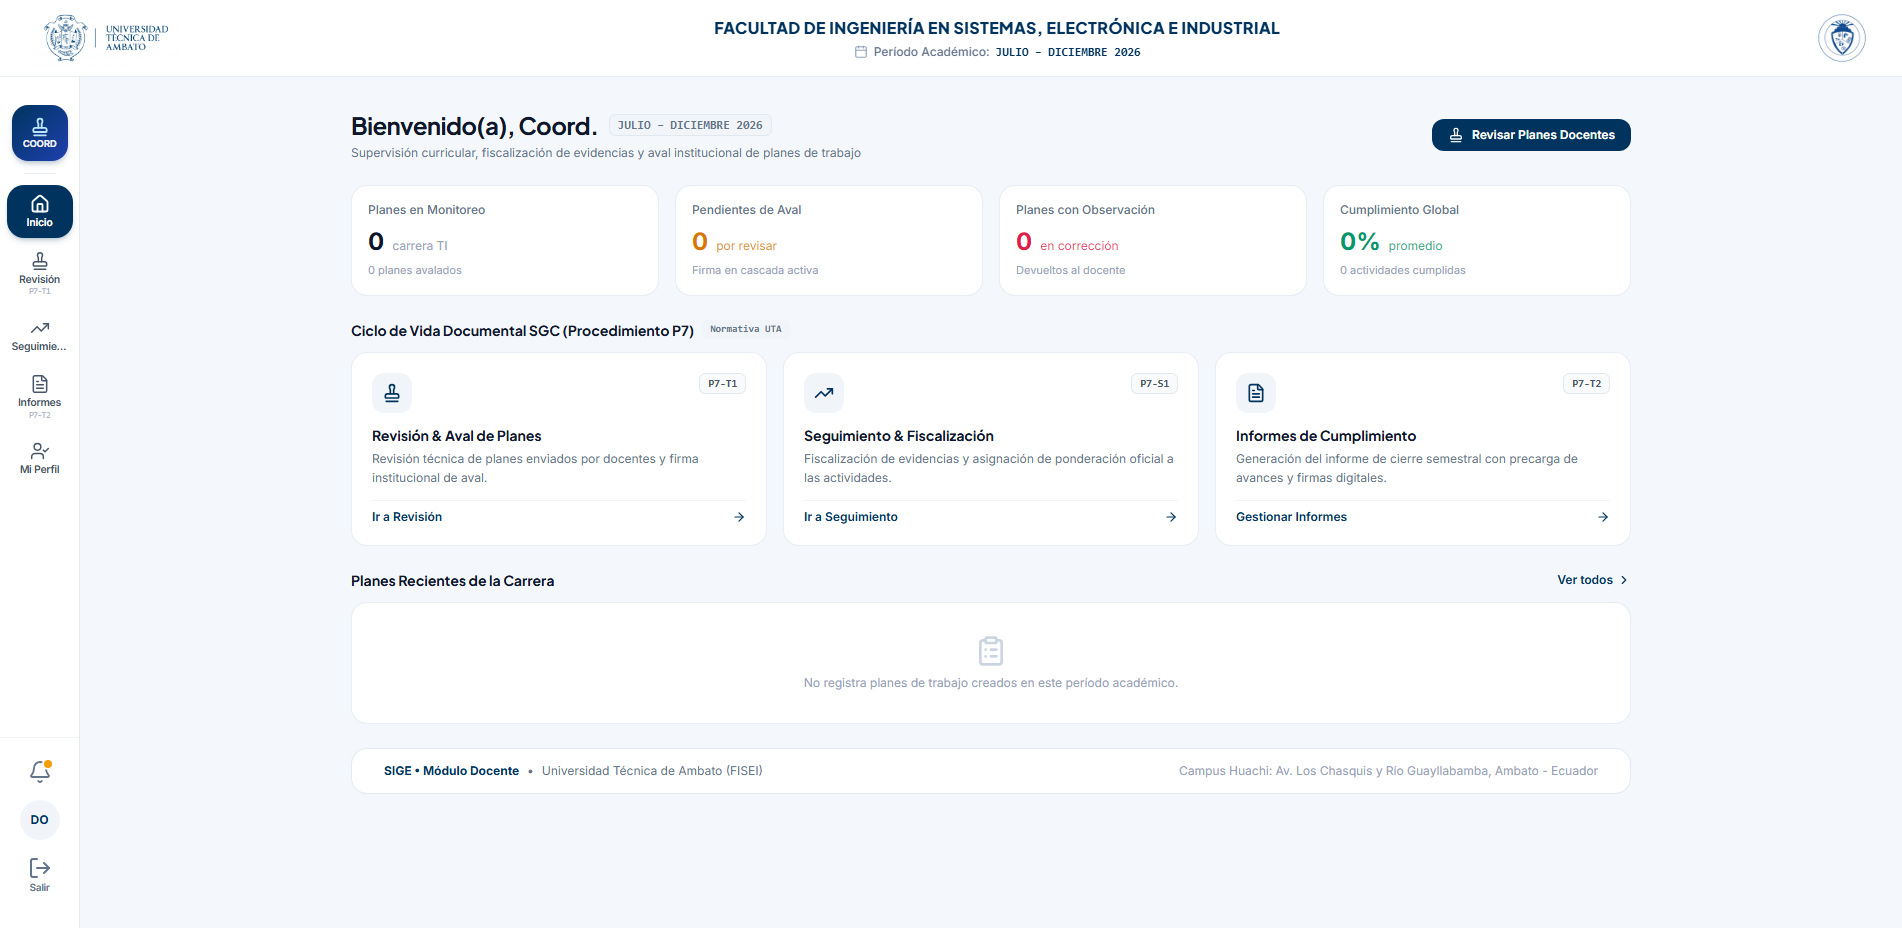
\includegraphics[width=0.88\textwidth,height=5.8cm,keepaspectratio]{images/sige_coordinador_revision.png}
    \caption{Captura Real del Panel de Revisión del Coordinador con Drawer de Observaciones en SIGE.}
    \label{fig:coordinador_real}
\end{figure}
\FloatBarrier

\begin{figure}[H]
    \centering
    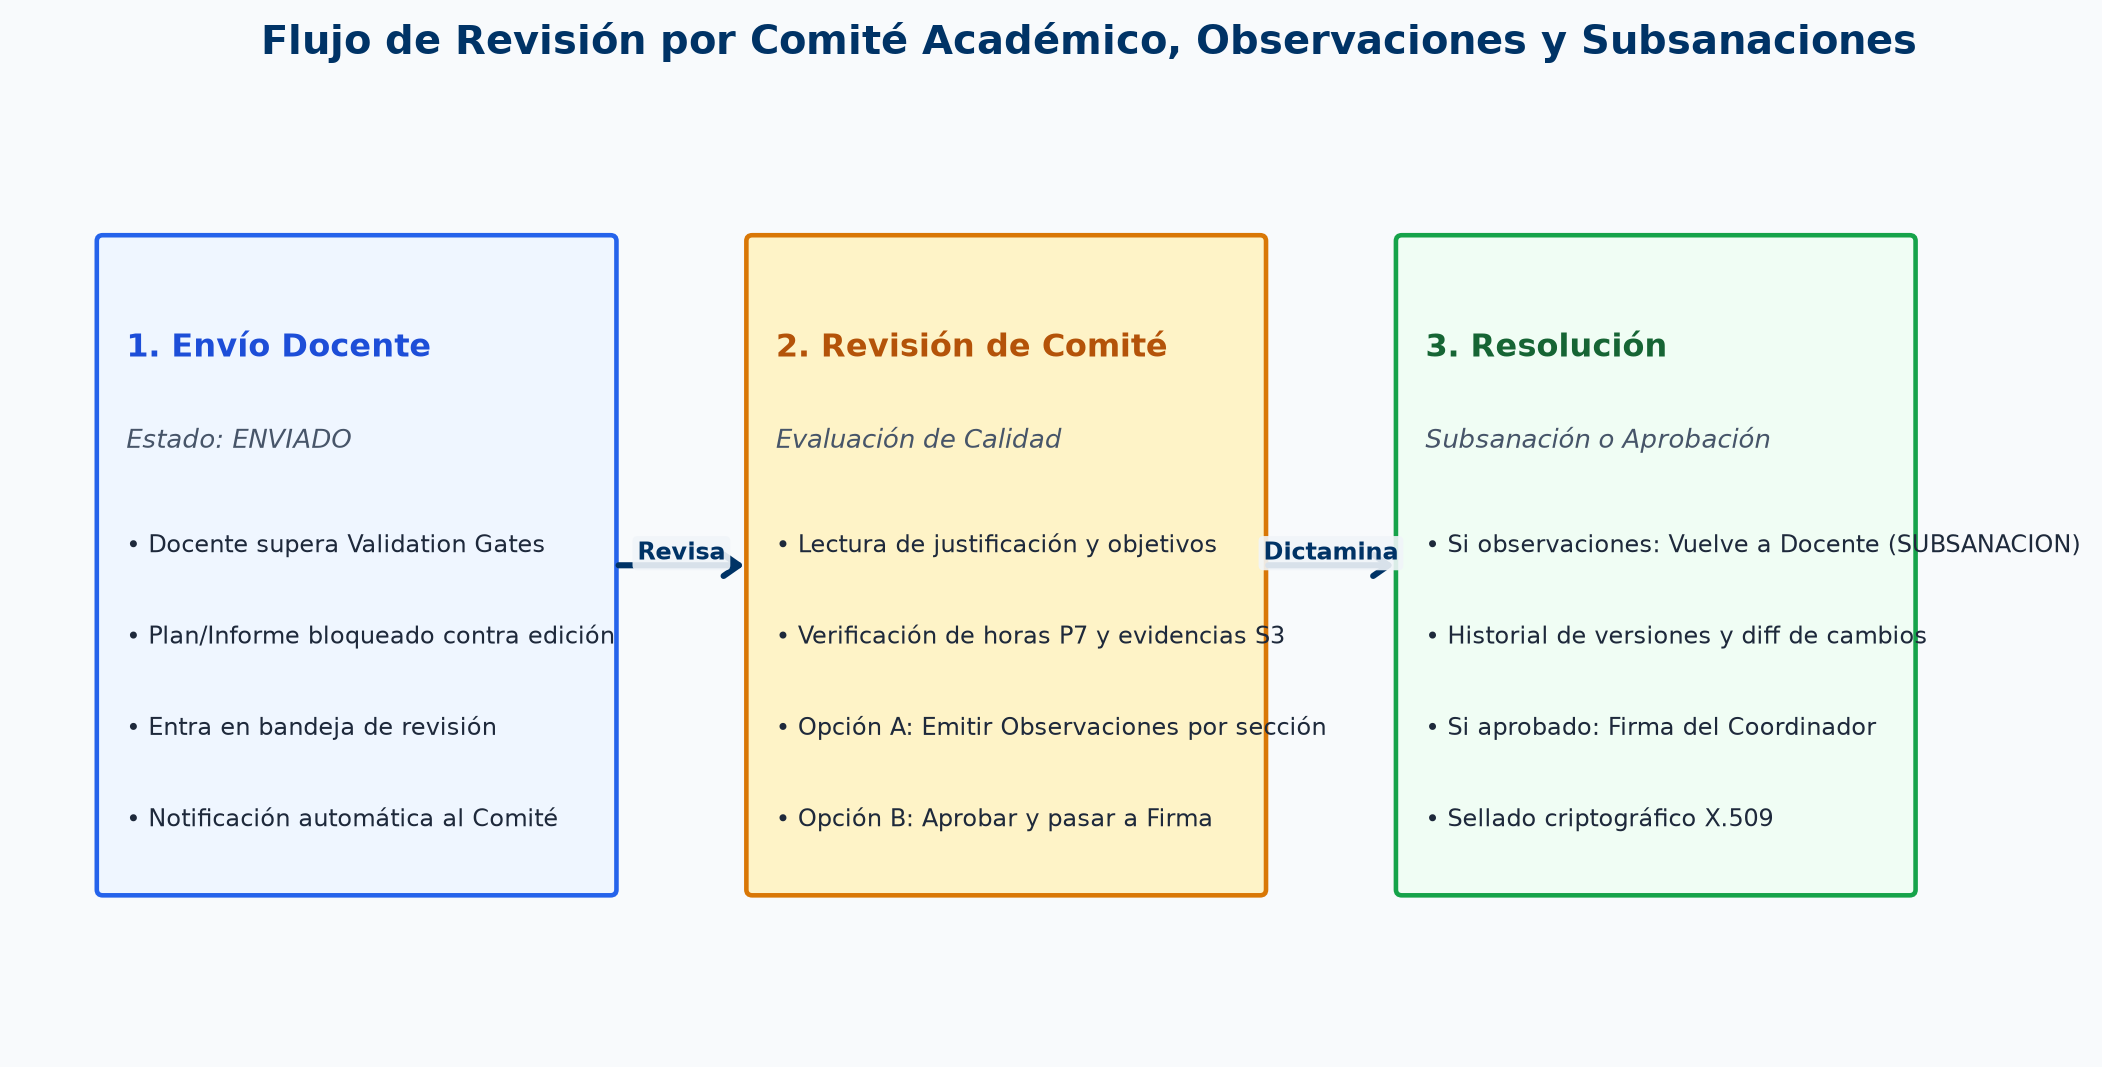
\includegraphics[width=0.88\textwidth,height=5.6cm,keepaspectratio]{images/f3_11_flujo_revision_comite.png}
    \caption{Flujo Secuencial de Estados y Cascada de Firmas Digitales en el Sistema SIGE.}
    \label{fig:cascada_firmas}
\end{figure}
\FloatBarrier

\section{Descripción de actividades}
\subsection{Matriz de la Cascada de Firmas Digitales Institucionales}
\begin{table}[H]
\centering
\small
\renewcommand{\arraystretch}{1.2}
\begin{tabularx}{\textwidth}{|c|>{\raggedright\arraybackslash\bfseries}m{2.8cm}|m{2.8cm}|X|c|}
\hline
\rowcolor{tableheader}
\textbf{Orden} & \textbf{Nivel de Firma} & \textbf{Actor Responsable} & \textbf{Efecto Jurídico y en el Sistema} & \textbf{Estado Resultante} \\
\hline
1 & Firma de Elaboración & Docente Titular / Ocasional & Certifica la veracidad de horas y actividades; bloquea edición. & \textbf{En Revisión} \\
\hline
2 & Firma de Revisión & Coordinador de Área / Carrera & Certifica cumplimiento técnico SGC y ausencia de observaciones. & \textbf{Aprobado Comisión} \\
\hline
3 & Firma de Aprobación & Subdecano de FISEI & Legalización oficial en Consejo Directivo; sella plan definitivo. & \textbf{Aprobado HCD (Final)} \\
\hline
\end{tabularx}
\caption{Matriz oficial de la cascada de firmas digitales multinivel.}
\label{tab:firmas_matrix}
\end{table}

\subsection{Matriz de Ciclo de Vida de las Observaciones Granulares}
\begin{table}[H]
\centering
\small
\renewcommand{\arraystretch}{1.2}
\begin{tabularx}{\textwidth}{|>{\bfseries}m{3.2cm}|m{3.0cm}|X|c|}
\hline
\rowcolor{tableheader}
\textbf{Severidad} & \textbf{Impacto en Flujo} & \textbf{Tratamiento en la Interfaz} & \textbf{Acción del Docente} \\
\hline
Informativa & No bloqueante & Sugerencia tipográfica menor; no impide avance a firma. & Opcional \\
\hline
Revisión Técnica & Bloqueante & Exige corrección en sección de horas o medios de verificación. & Obligatoria \\
\hline
Rechazo Normativo & Bloqueante Mayor & Devuelve expediente a estado ``Observado'' de forma inmediata. & Reestructuración \\
\hline
\end{tabularx}
\caption{Clasificación y comportamiento de observaciones de revisión.}
\end{table}

\section{Firmas de Responsabilidad}

\noindent
\renewcommand{\arraystretch}{1.2}
\begin{tabularx}{\textwidth}{|>{\raggedright\arraybackslash}m{2.9cm}|>{\raggedright\arraybackslash}X|>{\centering\arraybackslash}m{4.6cm}|>{\centering\arraybackslash}m{2.3cm}|}
    \hline
    \rowcolor{tableheader}
    \textbf{ACCIÓN} & \textbf{NOMBRE Y CARGO} & \textbf{FIRMA} & \textbf{FECHA} \\
    \hline
    \textbf{Elaborado por:} & Heidi Villavicencio\newline Analista de Calidad / UI-UX & \parbox[c]{4.4cm}{\centering\vspace{4pt}
\includegraphics[height=1.5cm,width=4.0cm,keepaspectratio]{images/firma_heidi.png}\vspace{4pt}} & 06/10/2026 \\
    \hline
    \textbf{Revisado por:} & Steeven Toala\newline Líder de Proyecto / Arquitecto & \parbox[c]{4.4cm}{\centering\vspace{4pt}
\includegraphics[height=1.5cm,width=4.0cm,keepaspectratio]{images/firma_steveen.png}\vspace{4pt}} & 06/10/2026 \\
    \hline
    \textbf{Aprobado por:} & Ing. Paulo Torres, Mg.\newline Docente Evaluador -- Gestión Proyectos & \parbox[c]{4.4cm}{\centering\vspace{8pt}\textbf{\textcolor{gray!80}{\scriptsize [ PENDIENTE DE APROBACIÓN ]}}\vspace{8pt}} & \textbf{\textcolor{gray!90}{Pendiente}} \\
    \hline
\end{tabularx}

\vspace{0.4cm}

\section{Control de Cambios}

\noindent
\renewcommand{\arraystretch}{1.2}
\begin{tabularx}{\textwidth}{|>{\hsize=0.45\hsize\centering\arraybackslash}X|>{\hsize=1.55\hsize\raggedright\arraybackslash}X|>{\hsize=1.2\hsize\raggedright\arraybackslash}X|>{\hsize=0.8\hsize\centering\arraybackslash}X|}
    \hline
    \rowcolor{tableheader}
    \textbf{Versión} & \textbf{Descripción del cambio} & \textbf{Responsable del cambio} & \textbf{Fecha de aprobación} \\
    \hline
    1.0 & Emisión inicial del entregable según EDT del Tablero Trello & Equipo de Proyecto SIGE & 06/10/2026 \\
    \hline
\end{tabularx}

\vspace{0.4cm}

\section{Anexos}

\subsection*{Anexo 1: Ficha Técnica de la Tarea EDT 3.13 en el Tablero Trello}
\begin{table}[H]
\centering
\small
\renewcommand{\arraystretch}{1.2}
\begin{tabularx}{\textwidth}{|>{\bfseries}m{3.5cm}|X|}
\hline
\rowcolor{tableheader}
\textbf{Parámetro EDT} & \textbf{Detalle Oficial del Tablero Trello} \\
\hline
Código de Tarea & EDT 3.13 \\
\hline
Nombre de la Tarjeta & Módulo de Revisión, Observaciones y Cascada de Firmas \\
\hline
Fase Correspondiente & FASE 3. IMPLEMENTACIÓN Y DESARROLLO \\
\hline
Período de Ejecución & 02 de octubre al 06 de octubre de 2026 (3 días laborables) \\
\hline
Horas Asignadas & 24 horas hombre netas \\
\hline
Responsables Técnicos & Steeven Toala (ST), Heidi Villavicencio (HV) \\
\hline
Entregable Oficial & Panel de Comité y servicio de Firmas multinivel \\
\hline
Estado en el Tablero & 100\% Completado y Verificado en Sprint 4 \\
\hline
\end{tabularx}
\caption{Ficha técnica de la tarea EDT 3.13 en el Tablero Trello.}
\end{table}

\subsection*{Anexo 2: Matriz de Verificación de Integridad de Firmas Digitales}
\begin{table}[H]
\centering
\footnotesize
\renewcommand{\arraystretch}{1.15}
\begin{tabularx}{\textwidth}{|c|m{2.5cm}|X|c|}
\hline
\rowcolor{tableheader}
\textbf{Prueba} & \textbf{Condición Forzada} & \textbf{Respuesta del Subsistema Criptográfico} & \textbf{Resultado} \\
\hline
P1 - Salto de Nivel & Coordinador intenta firmar plan sin firma de docente & \texttt{ERROR: Cascada violada. Requiere firma de Elaborador} & BLOQUEADO \\
\hline
P2 - Alteración Posterior & Modificación manual de texto en base de datos tras firma & \texttt{ALERTA: Hash de contenido no coincide con firma (Corrupción)} & DETECTADO \\
\hline
P3 - Firma Legítima & Secuencia en orden con observaciones resueltas & Estampado con hash SHA-256 e inserción inmutable & EXITOSO \\
\hline
\end{tabularx}
\caption{Pruebas de integridad criptográfica y cascada de firmas.}
\end{table}

\subsection*{Anexo 3: Lista de Chequeo y Criterios de Aceptación Institucional (SGC ISO 9001:2015)}
\begin{table}[H]
\centering
\footnotesize
\renewcommand{\arraystretch}{1.15}
\begin{tabularx}{\textwidth}{|m{3.2cm}|X|c|c|}
\hline
\rowcolor{tableheader}
\textbf{Criterio de Calidad SGC} & \textbf{Mecanismo de Verificación Técnica} & \textbf{Conformidad} & \textbf{Responsable} \\
\hline
Cascada de Firmas & Secuencia institucional inmutable: Docente -> Coordinador -> Subdecano & 100\% CONFORME & Steeven Toala \\
\hline
Drawer de Observaciones & Panel lateral para registrar observaciones granulares por cada sección & 100\% CONFORME & Andrea Vásquez \\
\hline
Control de Transiciones & Cambio de estado a Observado con notificación inmediata al docente & 100\% CONFORME & Nixon Hurtado \\
\hline
Sellado Criptográfico & Estampado de firma digital SHA-256 vinculada a la cuenta del firmante & 100\% CONFORME & Heidi Villavicencio \\
\hline
\end{tabularx}
\caption{Lista de verificación y control de calidad institucional del entregable 3.13.}
\end{table}


\end{document}
